{\color{ggreen}\subsection{Regolarizzazione del Metodo del Gradiente Coniugato \code{minimize}}}
In linea generale vediamo che al crescere dei $\lambda$, il PSNR fino a $\lambda \simeq 0.02$ 
continua ad aumentare, 
quindi migliora l'immagine, raggiunge un picco massimo e successivamente decresce.
Quindi deduciamo che tramite la regolarizzazione si ottiene una soluzione o un PSNR migliore, ma non per 
qualsiasi valore di $\lambda$. 

{\color{ggreen}\subsubsection{Immagini geometriche regolarizzate}}
Grafici andamento PSNR, media PSNR e MSE nella ricostruzione delle immagini con il metodo di regolarizzazione:

\begin{figure}[H]
    \centering
    \begin{subfigure}{0.5\textwidth}
        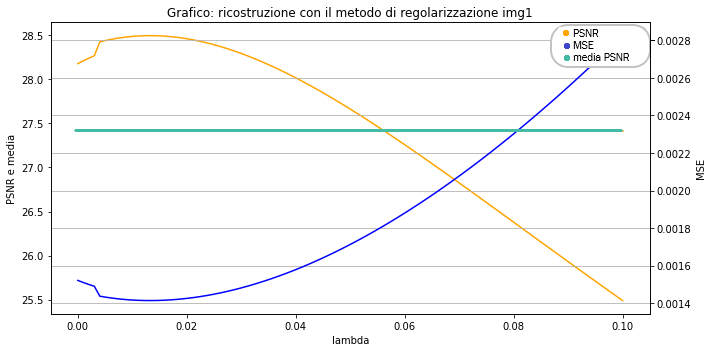
\includegraphics[width=\textwidth]{imgRicostruzione/grafico1minimize.png}
    \end{subfigure}%
    \begin{subfigure}{0.5\textwidth}
        \centering
        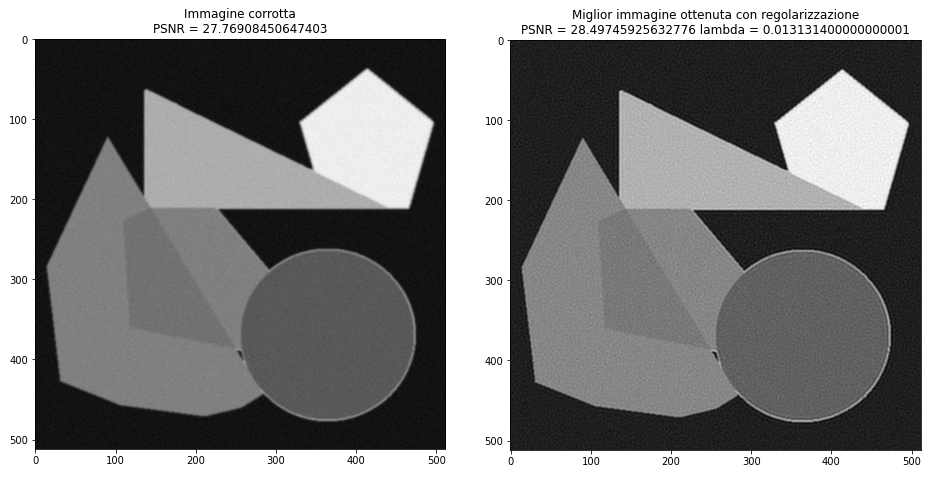
\includegraphics[width=\textwidth]{imgRicostruzione/ricostruzione1minimize.png}
    \end{subfigure}
    \caption{Ricostruzione immagine geometrica img1.png [a destra: immagine corrotta, sinistra: miglior immagine ottenuta con regolarizzazione]}
    
    \begin{subfigure}{0.5\textwidth}
        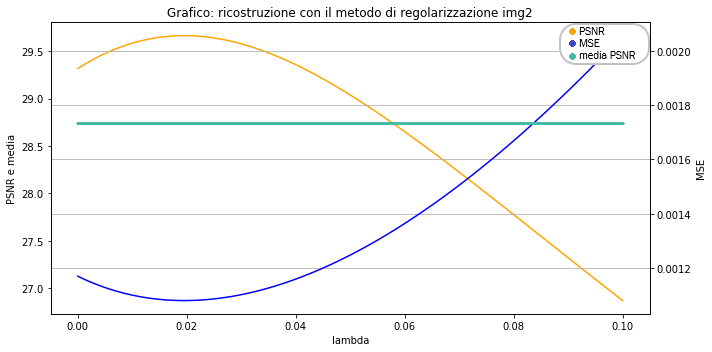
\includegraphics[width=\textwidth]{imgRicostruzione/grafico2minimize.png}
    \end{subfigure}%
    \begin{subfigure}{0.5\textwidth}
        \centering
        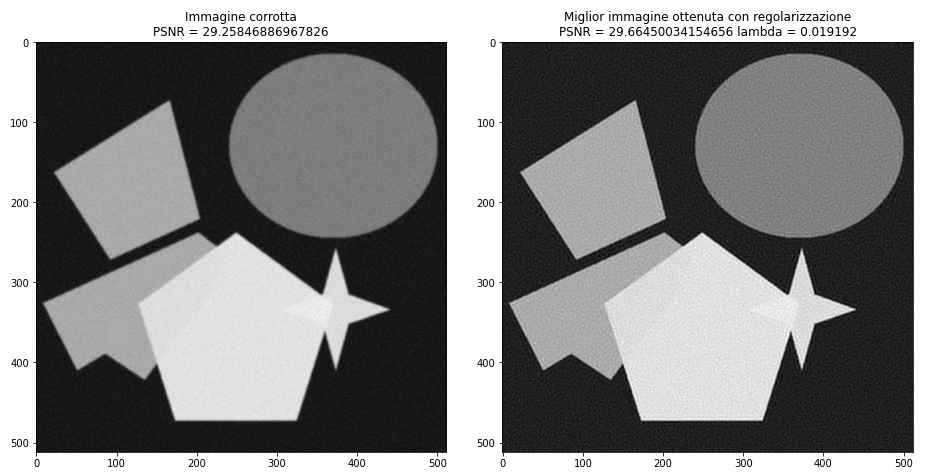
\includegraphics[width=\textwidth]{imgRicostruzione/ricostruzione2minimize.png}
    \end{subfigure}
    \caption{Ricostruzione immagine geometrica img2.png [a destra: immagine corrotta, sinistra: miglior immagine ottenuta con regolarizzazione]}
    
    \begin{subfigure}{0.5\textwidth}
        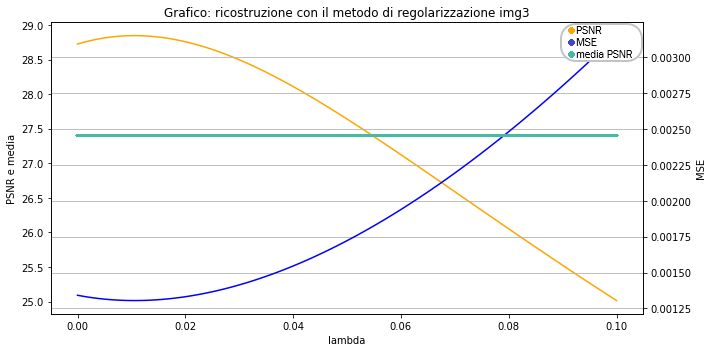
\includegraphics[width=\textwidth]{imgRicostruzione/grafico3minimize.png}
    \end{subfigure}%
    \begin{subfigure}{0.5\textwidth}
        \centering
        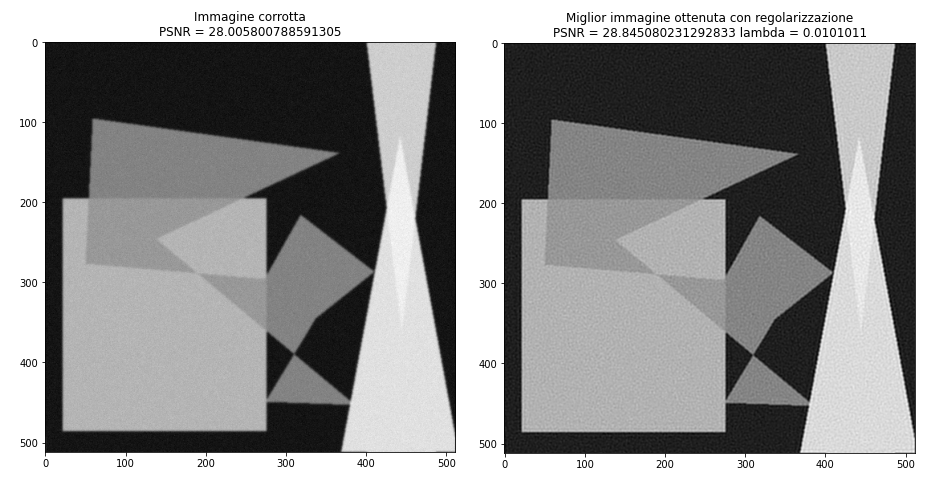
\includegraphics[width=\textwidth]{imgRicostruzione/ricostruzione3minimize.png}
    \end{subfigure}
    \caption{Ricostruzione immagine geometrica img3.png [a destra: immagine corrotta, sinistra: miglior immagine ottenuta con regolarizzazione]}
\end{figure}
\begin{figure}[H]
    \centering
    \begin{subfigure}{0.5\textwidth}
        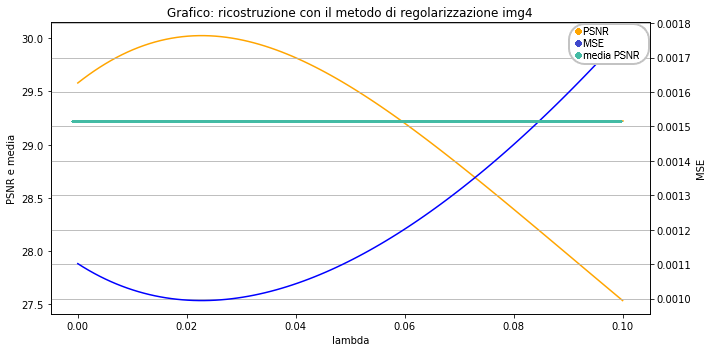
\includegraphics[width=\textwidth]{imgRicostruzione/grafico4minimize.png}
    \end{subfigure}%
    \begin{subfigure}{0.5\textwidth}
        \centering
        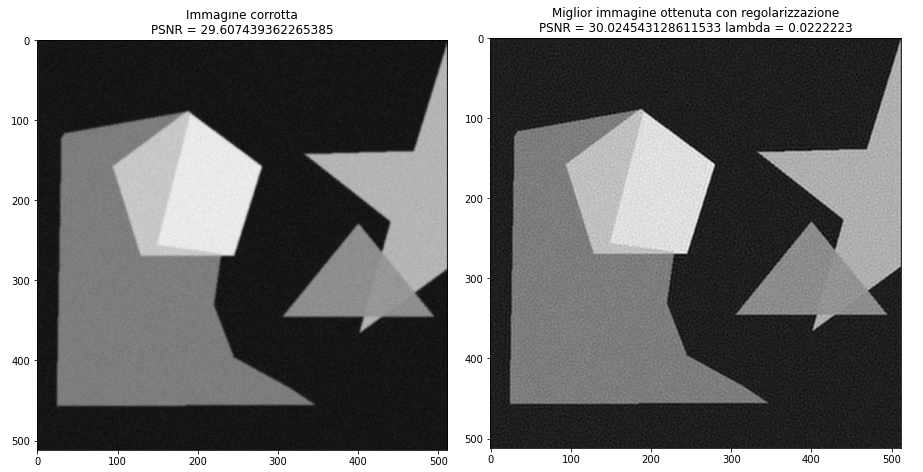
\includegraphics[width=\textwidth]{imgRicostruzione/ricostruzione4minimize.png}
    \end{subfigure}
    \caption{Ricostruzione immagine geometrica img4.png [a destra: immagine corrotta, sinistra: miglior immagine ottenuta con regolarizzazione]}

    \begin{subfigure}{0.5\textwidth}
        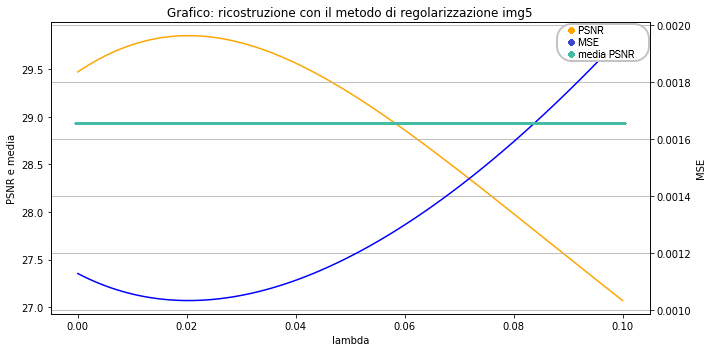
\includegraphics[width=\textwidth]{imgRicostruzione/grafico5minimize.png}
    \end{subfigure}%
    \begin{subfigure}{0.5\textwidth}
        \centering
        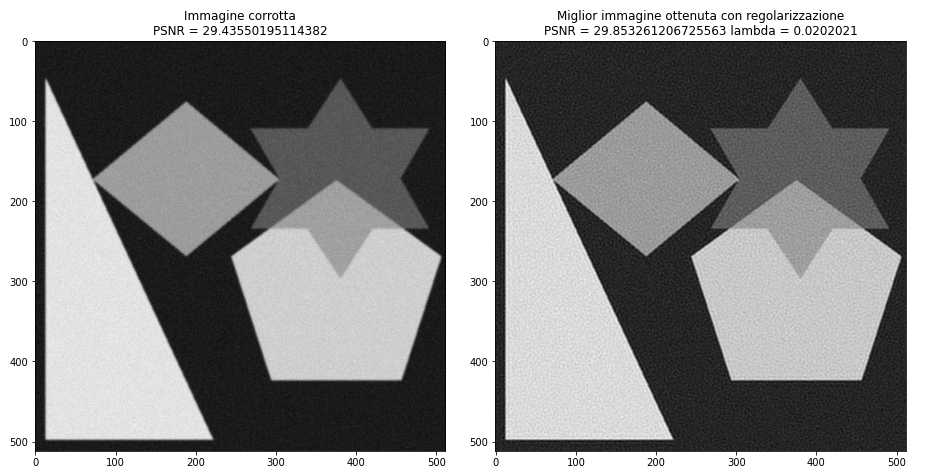
\includegraphics[width=\textwidth]{imgRicostruzione/ricostruzione5minimize.png}
    \end{subfigure}
    \caption{Ricostruzione immagine geometrica img5.png [a destra: immagine corrotta, sinistra: miglior immagine ottenuta con regolarizzazione]}
    
    \begin{subfigure}{0.5\textwidth}
        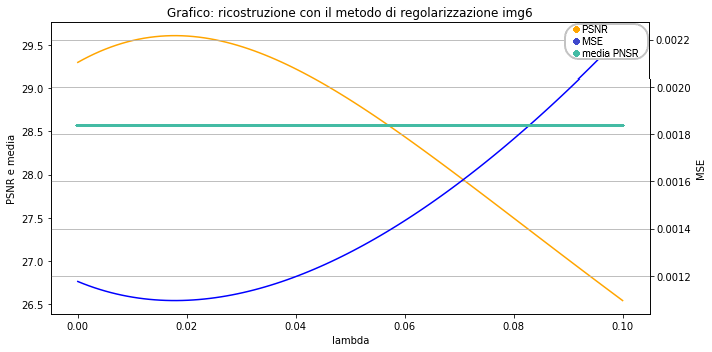
\includegraphics[width=\textwidth]{imgRicostruzione/grafico6minimize.png}
    \end{subfigure}%
    \begin{subfigure}{0.5\textwidth}
        \centering
        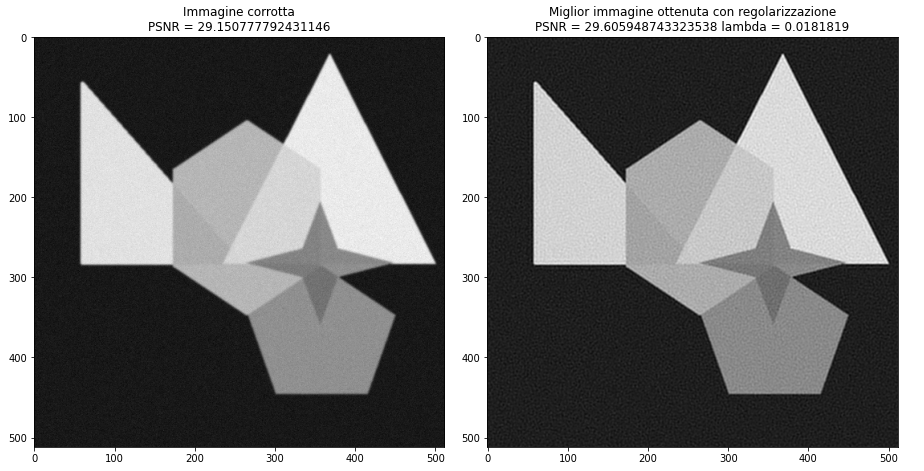
\includegraphics[width=\textwidth]{imgRicostruzione/ricostruzione6minimize.png}
    \end{subfigure}
    \caption{Ricostruzione immagine geometrica img6.png [a destra: immagine corrotta, sinistra: miglior immagine ottenuta con regolarizzazione]}
    
    \begin{subfigure}{0.5\textwidth}
        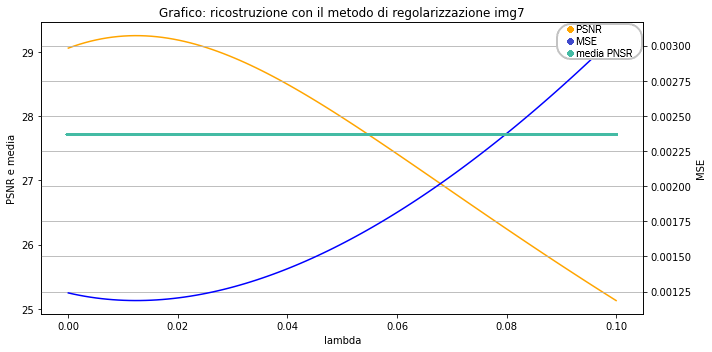
\includegraphics[width=\textwidth]{imgRicostruzione/grafico7minimize.png}
    \end{subfigure}%
    \begin{subfigure}{0.5\textwidth}
        \centering
        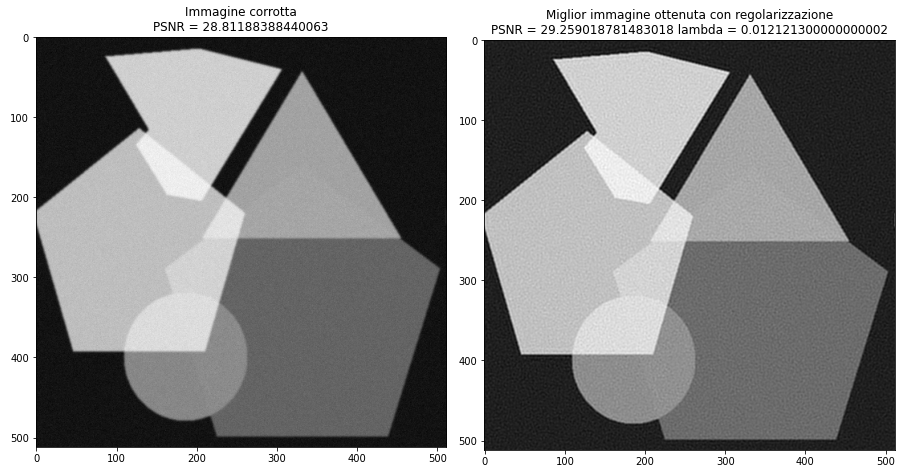
\includegraphics[width=\textwidth]{imgRicostruzione/ricostruzione7minimize.png}
    \end{subfigure}
    \caption{Ricostruzione immagine geometrica img7.png [a destra: immagine corrotta, sinistra: miglior immagine ottenuta con regolarizzazione]}
\end{figure}
\begin{figure}[H]
    \centering
    \begin{subfigure}{0.5\textwidth}
        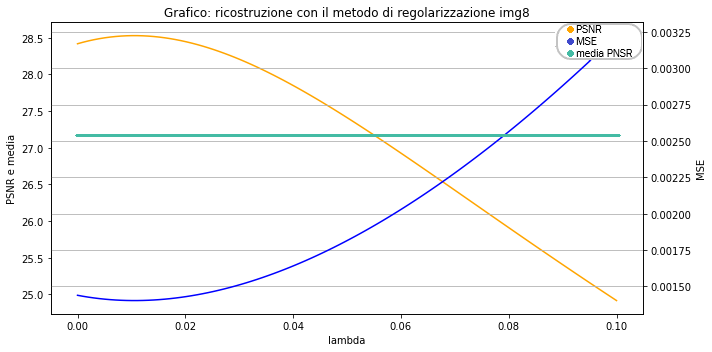
\includegraphics[width=\textwidth]{imgRicostruzione/grafico8minimize.png}
    \end{subfigure}%
    \begin{subfigure}{0.5\textwidth}
        \centering
        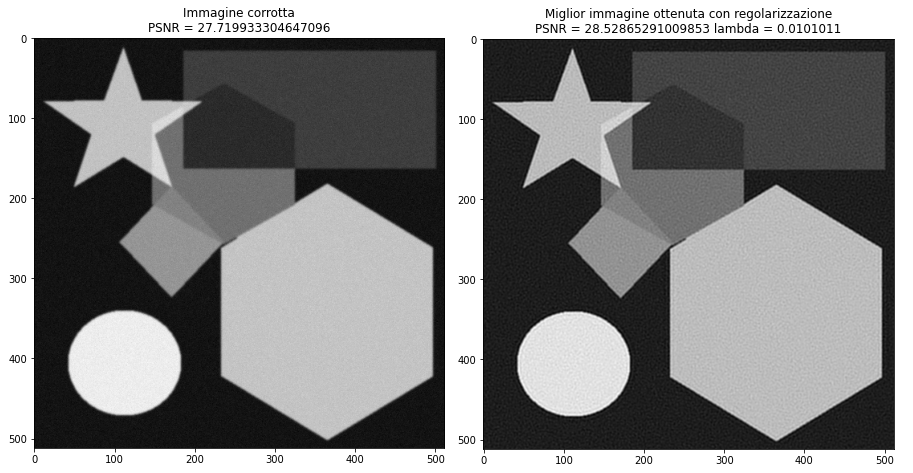
\includegraphics[width=\textwidth]{imgRicostruzione/ricostruzione8minimize.png}
    \end{subfigure}
    \caption{Ricostruzione immagine geometrica img8.png [a destra: immagine corrotta, sinistra: miglior immagine ottenuta con regolarizzazione]}
\end{figure}

{\color{ggreen}\subsubsection{Immagini fotografiche regolarizzate}}
\begin{figure}[H]
    \centering
    \begin{subfigure}{0.5\textwidth}
        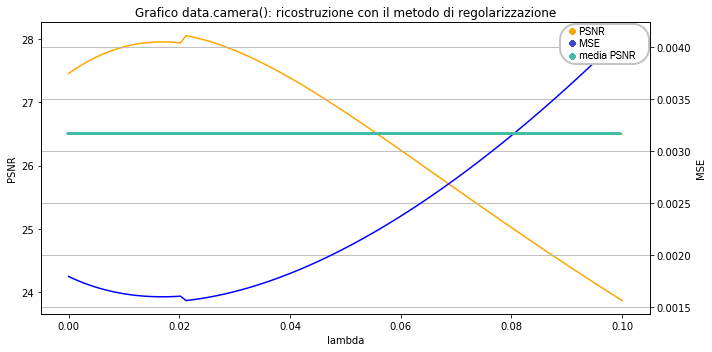
\includegraphics[width=\textwidth]{imgRicostruzione/graficoCameraman_minimize.png}
    \end{subfigure}%
    \begin{subfigure}{0.5\textwidth}
        \centering
        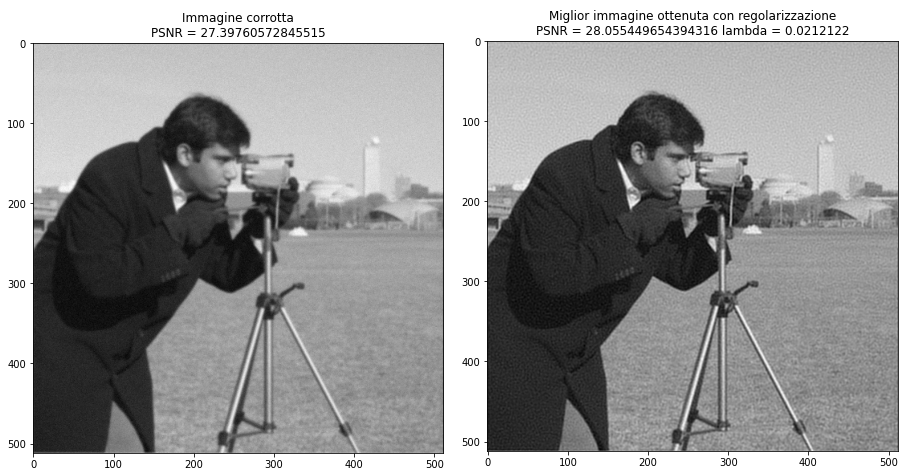
\includegraphics[width=\textwidth]{imgRicostruzione/ricostruzioneCameraman_minimize.png}
    \end{subfigure}
    \caption{Ricostruzione immagine fotografica data.camera() [a destra: immagine corrotta, sinistra: miglior immagine ottenuta con regolarizzazione]}
    
    \centering
    \begin{subfigure}{0.5\textwidth}
        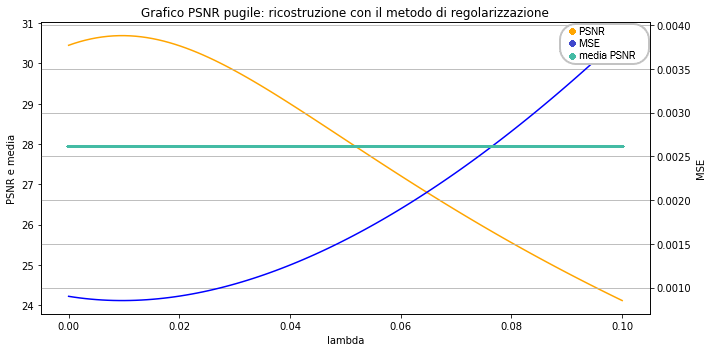
\includegraphics[width=\textwidth]{imgRicostruzione/graficoPugile_minimize.png}
    \end{subfigure}%
    \begin{subfigure}{0.5\textwidth}
        \centering
        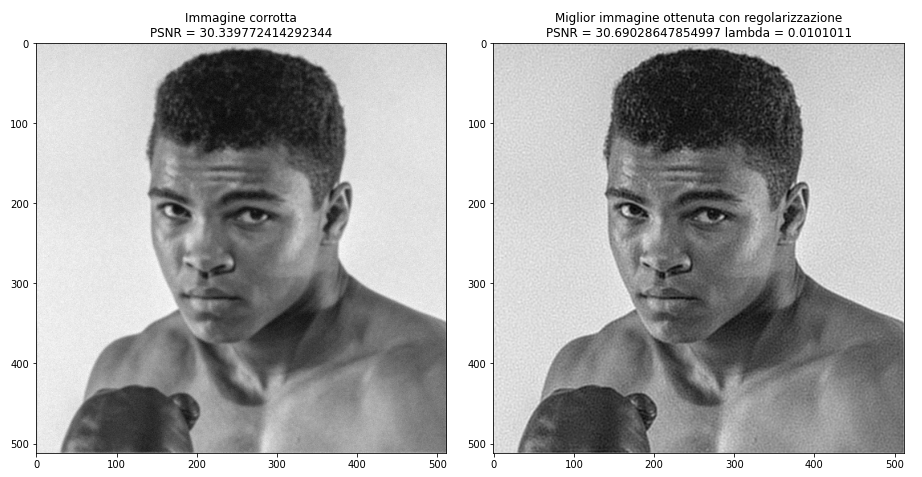
\includegraphics[width=\textwidth]{imgRicostruzione/ricostruzionePugile_minimize.png}
    \end{subfigure}
    \caption{Ricostruzione immagine fotografica pugile.png [a destra: immagine corrotta, sinistra: miglior immagine ottenuta con regolarizzazione]}
\end{figure}